% =======================================================================
% OUTDATED DRAFT (superseded 2026-10-29). Kept for reference only; do not edit.
% This version argues that taxonomy conditioning is a "precision regularizer,
% not a mode selector". The reset-pose probe (eval_results/reset_pose_probe.py)
% showed the opposite: at deployment the label acts as a mode selector (switch).
% The current paper is paper.tex (RA-L format).
% =======================================================================
\documentclass[11pt]{article}

\usepackage[margin=1in]{geometry}
\usepackage[T1]{fontenc}
\usepackage{lmodern}
\usepackage{microtype}
\usepackage{amsmath,amssymb}
\usepackage{booktabs}
\usepackage{graphicx}
\usepackage{xcolor}
\usepackage{enumitem}
\usepackage{placeins}
\usepackage{tikz}
\usetikzlibrary{positioning,arrows.meta,fit,calc}
\usepackage{hyperref}
\usepackage[numbers,sort&compress]{natbib}

\graphicspath{{figures/}}

% Convenience macro for TODO markers left in the manuscript during drafting.
\newcommand{\todo}[1]{\textcolor{red}{\textbf{[TODO:} #1\textbf{]}}}

\title{CRAG: Classifier-Regularized Action Generation for Dexterous Climbing-Hold Grasps}
\author{Anonymous Authors}
\date{}

\begin{document}
\maketitle

\noindent\fbox{\parbox{\dimexpr\linewidth-2\fboxsep-2\fboxrule}{\color{red}\textbf{Outdated
draft (superseded October 2026).} The mechanistic claims below (taxonomy as a
precision regularizer, not a mode selector) are no longer supported. See the current
RA-L version, \texttt{paper.tex}.}}

\begin{abstract}

Dexterous grasping in robotics relies on distinct hand configurations depending on object geometry. In our testbed of rock climbing holds this becomes evident in styles of holds, for thin edges a crimp is required, for slopers an open hand press is required, etc. Existing diffusion-policy approaches learn the singular action distribution per task, but don't model grasp taxonomy. This leaves the question of how taxonomy conditioning will impact the learned distribution. We introduce \textbf{CRAG}, a grasp-taxonomy-conditioned 3D diffusion policy that builds off a DP3-style point-cloud policy on a four-class label (crimp, sloper, pinch, and jug) for a Franka arm with a 16-DoF LEAP hand end effector. This is done in conjunction with a climbing-hold manipulation benchmark on a spring-constrained displacement testbed with a linear ratchet that produces a slip-force readout in newtons, evaluated at five orientations ($0^\circ$, $\pm 22.5^\circ$, $\pm 45^\circ$).

The trained models we evaluated showed that the system without grasp-taxonomy does not have any classical mode collapse. The latent representation of the holds already separates grasp types (kNN accuracy 99\%, silhouette score 0.32), and its mean predicted actions differ by 90\% of the demonstrator's between type spread (0.316\,rad vs.0.352\,rad). The main benefit of taxonomy conditioning is \emph{precision}. In the diffusion decoder there is a 15--30\% lower within-input variance on grasp types. 

Hardware evaluation on 80 paired trials supports this mechanistic prediction. Taxonomy conditioning improves median slip force by +5.2\,N (Wilcoxon signed-rank, $p < 0.001$, Cohen's $d = 0.95$), with effect sizes ordered by contact-tolerance tightness: $d = 1.82$ on pinch (a 20-of-20 paired-win count), $d = 1.08$ on sloper, $d = 1.05$ on crimp, and $d = 0.55$ on jug
The system's failure mode was grasps slipping on holds, this drops from 44\% of trials without grasp taxonomy to 10\% with grasp taxonomy. To our knowledge, CRAG is the first imitation-learning execution policy to condition on grasp taxonomy for a dexterous hand and arm system with multiple degrees of freedom, and the first to mechanistically characterize what this conditioning does to the action distribution.
\end{abstract}

% -----------------------------------------------------------------------
\section{Introduction}
% -----------------------------------------------------------------------

\begin{figure}[!ht]
\centering
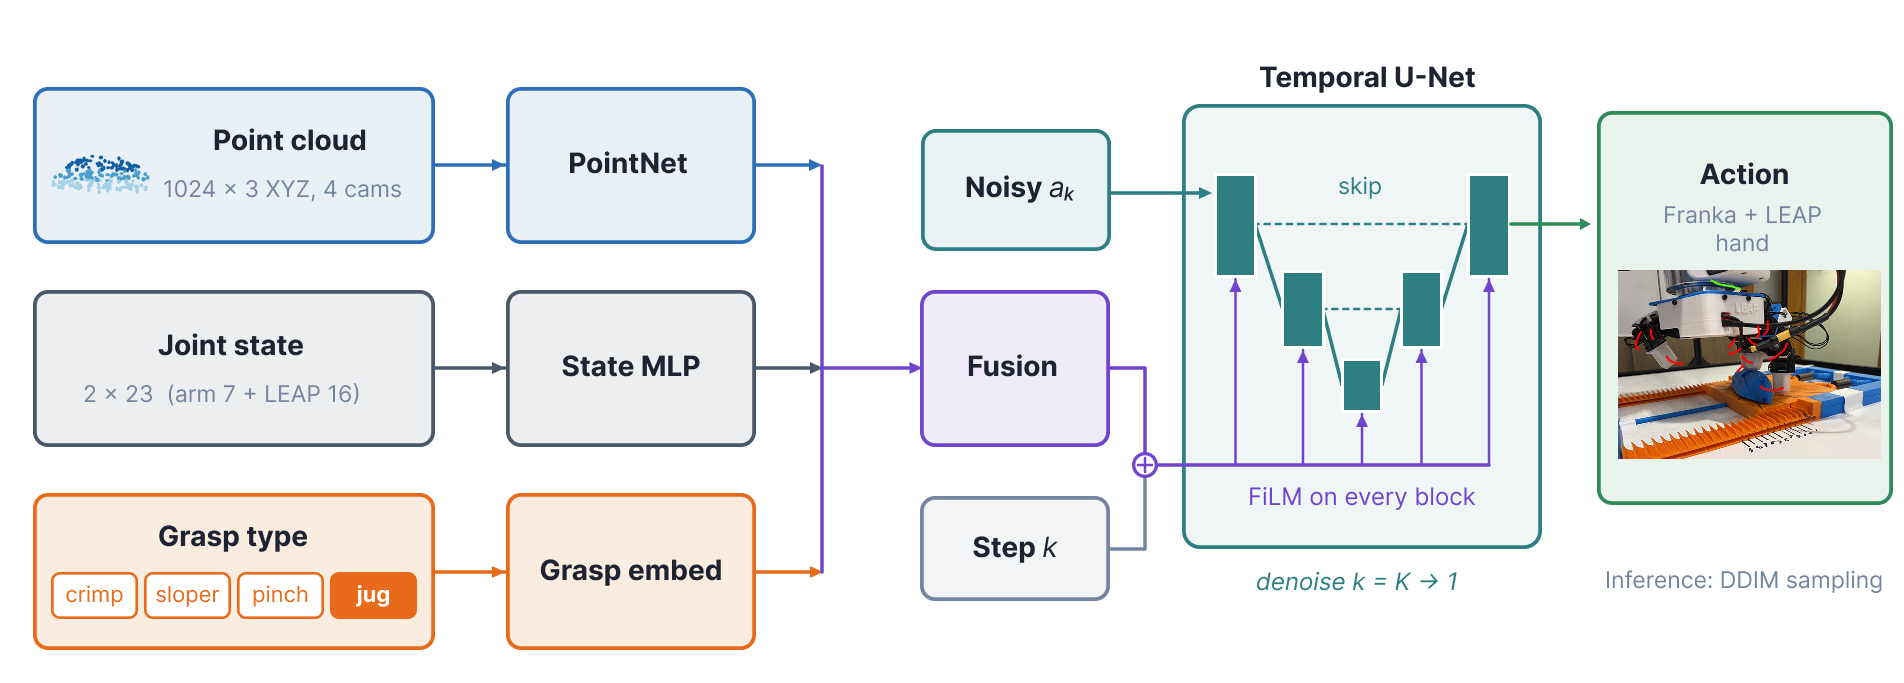
\includegraphics[width=\textwidth]{fig_architecture.png}
\caption{CRAG architecture. Point cloud, proprioception, and grasp-type
label are encoded independently and fused into a 512-d conditioning vector $z$
that feature-wise conditions a 1D temporal U-Net diffusion denoiser. The
without-taxonomy ablation drops only the grasp-type branch (orange)
(37{,}248 parameters, $0.1\%$ of 34.6\,M).}
\label{fig:arch}
\end{figure}

Imitation learning based manipulation has developed rapidly on parallel-jaw claw grippers. Development on multi-finger end effectors has been slower to follow, because the subtle changes in object geometry require equally subtle changes in hand finger formations. Within the domain of climbing holds the way and grip created to grasp onto a hold directly determines how much force a grip can exert before slipping off. In this paper we split the same high level task (``grasp the hold'') into 4 distinct strategies: \emph{crimp} (tight curled fingertips on thin edges), \emph{sloper} (open-hand full contact frictional pressing), \emph{pinch} (thumb-ulnar finger opposition), and \emph{jug} (ulnar digits grasp incut handles). Each of these grasp strategies correspond to different feasible hand positions and contact spaces, with different failure modes under load.

Diffusion-based behavior cloning has become the standard for visuomotor policy learning \citep{chi2023diffusionpolicy,ho2020ddpm}. We built on top of DP3 \citep{ze2024dp3}, a 3D diffusion policy that operates on point clouds, as our base architecture (Fig.~\ref{fig:arch}). The problem arises for multi-grasp policies in how grasping distribution is mapped out. Most diffusion policies treat grasping as a single distribution conditioned on observations. These observations from point-clouds alone lack explicit conditioning on grasp taxonomy. Recent work on taxonomy-conditioned grasping \citep{dexonomy2025,tian2024graspasyousay} does train on grasp type but only generates static poses on an end effector, rather than executable autonomy trajectories, leaving execution-policy open.

The natural hypothesis is that taxonomy conditioning helps as a \emph{mode selector}. Without taxonomy a policy trained on multi grasp datasets could collapse to one grasp type and fail when faced with a mixed test set. In our example, it could collapse to, say, a jug grasp every time and fail for the other 3 grasping tasks. Our analysis rejects this theory. The non-taxonomy policy separates grasp types in its representation and produces actions that commit to four very distinct configurations, reaching 90\% of the training data's between-type spread. The taxonomy label acted as a precision regulator, reducing within-input sampling variability, creating a tighter diffusion decoder output distribution around the correct subtype. This prediction is testable on hardware: conditioning should help in cases where contact tolerances are precise (crimp, sloper, pinch), and where geometry is looser (jug). The empirical per-type success pattern follows suit.

\begin{figure}[t]
\centering
\includegraphics[width=0.65\textwidth]{fig_hero_grasp.jpg}
\caption{CRAG in action. The LEAP Hand v1 (16-DoF, on a Franka Emika
Panda) executes a taxonomy-conditioned grasp on a 3D-printed jug hold seated on
the spring-constrained displacement testbed. The orange ratchet teeth
(foreground) capture peak hold displacement during the post-grasp pull test,
converting evaluation from a binary lift outcome into a continuous slip-force
readout (N).}
\label{fig:hero}
\end{figure}

\paragraph{Contributions.}
\begin{enumerate}[leftmargin=*,topsep=2pt,itemsep=2pt]
  \item A \textbf{grasp-taxonomy-aware 3D diffusion policy} (CRAG) that
    conditions action diffusion on a grasp-type label alongside 3D point-cloud
    geometry and robot proprioception, built on DP3-style architectures
    \citep{ze2024dp3}.
  \item A \textbf{climbing-hold manipulation benchmark} with a spring-constrained
    displacement testbed and linear ratcheting mechanism, providing continuous
    grip-stability measurements across five hold orientations per grasp/hold type.
  \item A \textbf{mechanistic characterisation} showing that taxonomy conditioning
    acts as a precision regularizer (15--30\% within-input variance reduction on
    precision-critical types), not a mode selector, with evidence from latent-space
    analysis, action-distribution comparison, and per-type robot evaluation.
  \item A \textbf{paired evaluation protocol} with global model-order
    alternation and per-trial point-cloud capture, supporting Wilcoxon signed-rank
    inference and Cohen's $d$ on paired differences.
\end{enumerate}

% -----------------------------------------------------------------------
\section{Related Work}
% -----------------------------------------------------------------------
\subsection{Diffusion Policies for Robot Control}
Diffusion Policy \citep{chi2023diffusionpolicy} formulates behavior cloning as
conditional denoising. It's responsible for generating action trajectories via a temporal U-Net that is conditioned
on observations. This approach uses the multimodality of diffusion
models \citep{ho2020ddpm} and often accelerates inference with DDIM \citep{song2021ddim}.

DP3 \citep{ze2024dp3} builds on diffusion policy to extend its tooling to point-cloud observation inputs using a PointNet-style encoder \citep{qi2017pointnet}. The subsequent work extends this to larger backbones and
broader task families \citep{ze2024idp3}. Category-level generalization using 3D semantic fields has achieved substantial gains on unseen instances \citep{wang2024gendp}. Diffusion models have also
been applied to grasp synthesis and dexterous grasp generation \citep{weng2024dexdiffuser}.

\subsection{Dexterous Manipulation Data and Embodiments}
Collecting high-quality dexterous demonstrations is a major bottleneck. DexCap
\citep{wang2024dexcap} proposes scalable mocap-based pipelines for hand--arm systems,
providing practical guidance on sensors, calibration, and capture rates. Our setup
targets the same Franka + dexterous hand configuration. For teleoperation we build
directly on the open-source OpenVR codebase \citep{george2023openvr}, a VR-based system
for the Franka arm originally paired with an Allegro hand. Our modifications retarget
the hand interface from the Allegro to the LEAP Hand v1, which provides the wider
finger range of motion required for our four-class taxonomy (notably the MCP abduction
and thumb opposition needed to span crimp curling, sloper extension, and pinch). Functional pre-grasp manipulation has been studied via diffusion policy with
teacher-student distillation \citep{wu2024unidexfpm}. CrossDex \citep{crossdex2025} addresses cross-embodiment
generalization via eigengrasp representations---complementary to our work, which targets
qualitatively distinct grasps on a fixed embodiment.

\subsection{Grasp Taxonomy and Type-Conditioned Grasping}
Human grasp taxonomies organize grasps into discrete categories reflecting opposition
type, thumb position, and power vs.\ precision \citep{feix2016grasp}. Several recent
lines of work condition dexterous grasp generation on such categories but produce static
poses rather than executable policies.

Most closely related, \textbf{Dexonomy} \citep{dexonomy2025} conditions on the full
33-type GRASP taxonomy from single-view point clouds to synthesize dexterous grasp
poses for a Shadow Hand (82.3\% real-world success). Critically, Dexonomy is a static
grasp-pose generator: it produces three snapshots (pre-grasp, grasp, squeeze) handed to
a motion planner, with no imitation learning and no continuous trajectory execution. In
contrast, CRAG learns a continuous visuomotor execution policy from teleoperated
demonstrations and additionally characterizes what the taxonomy label does to the
learned distribution.

Language-conditioned grasp generation \citep{tian2024graspasyousay} similarly produces
static poses. OmniDexVLG \citep{omnidexvlg2024} uses a VLM to infer taxonomy type,
feeding a downstream pose generator. DexGraspVLA \citep{dexgraspvla2026} combines a VLM
planner with a diffusion execution policy, but the VLM selects \emph{which object} to
grasp rather than \emph{how}; no per-type trajectory specialization is learned.

To our knowledge, CRAG is the first system to condition a continuous
imitation-learning execution policy on grasp taxonomy for a multi-DoF arm--hand system,
and the first to characterise mechanistically what that conditioning does to the learned
distribution. Table~\ref{tab:novelty} summarises the positioning.

\begin{table}[h]
\centering\small
\setlength{\tabcolsep}{4pt}
\caption{Positioning along four axes: point cloud input, grasp-taxonomy
conditioning, continuous execution policy (vs.\ static pose generation), and
dexterous hand.}
\label{tab:novelty}
\begin{tabular}{lcccc}
\toprule
Method & PC & Taxonomy & Exec.\ policy & Dex.\ hand \\
\midrule
DP3 \citep{ze2024dp3}                       & \checkmark & ---        & \checkmark   & Allegro \\
Dexonomy \citep{dexonomy2025}               & \checkmark & 31 types   & pose-gen     & Shadow \\
Grasp as You Say \citep{tian2024graspasyousay} & \checkmark & language & pose-gen     & \checkmark \\
OmniDexVLG \citep{omnidexvlg2024}           & partial    & VLM        & pose-gen     & \checkmark \\
DexGraspVLA \citep{dexgraspvla2026}         & ---        & obj.\ ID   & \checkmark   & \checkmark \\
\textbf{CRAG}                         & \checkmark & 4-class    & \checkmark arm+hand & LEAP \\
\bottomrule
\end{tabular}
\end{table}

% -----------------------------------------------------------------------
\section{Method: Grasp-Taxonomy-Aware 3D Diffusion Policy}
\label{sec:method}
% -----------------------------------------------------------------------

\subsection{Problem Formulation}
We consider episodic manipulation of a static climbing hold on a tabletop workspace.
At each control step $t$, the policy observes (i) a fused point cloud
$P \in \mathbb{R}^{N \times 3}$ (captured once per episode after parking the arm out
of the cameras' field of view), (ii) a proprioceptive state history $s_{t-T_o+1:t}$
over observation horizon $T_o$, and (iii) a grasp-type label $g \in \{0,1,2,3\}$
corresponding to \{crimp, sloper, pinch, jug\}. The policy outputs a joint-space
action chunk $a_{t:t+T_p-1}$ over prediction horizon $T_p$; the controller executes
the first $T_a \le T_p$ steps before replanning. The label $g$ is provided manually
during data collection and at deployment time.

Following \citet{chi2023diffusionpolicy}, we model the conditional distribution over
action sequences as a denoising diffusion process:
\[
p\!\left(a_{t:t+T_p-1} \mid P,\, s_{t-T_o+1:t},\, g\right),
\]
learned from teleoperated demonstrations via supervised diffusion loss.

\subsection{Architecture}
\label{sec:arch}
Our policy follows the DP3 design pattern \citep{ze2024dp3}: a point-cloud encoder
produces a 3D scene embedding, fused with robot state and a grasp-type embedding to
condition a 1D temporal U-Net that parameterises the diffusion denoiser
(Fig.~\ref{fig:arch}).

\paragraph{Point cloud encoder.}
A PointNet-style encoder \citep{qi2017pointnet} (channels $3 \to 64 \to 128 \to 256$,
no T-Net, max-pool, linear projection) maps $P \in \mathbb{R}^{1024 \times 3}$ to a
256-dimensional feature vector $z_P$. We use XYZ-only points (no colour) to reduce
sensitivity to appearance and lighting \citep{ze2024dp3}.

\paragraph{State and grasp-type conditioning.}
Robot proprioception over $T_o = 2$ timesteps is embedded via an MLP to obtain
$z_s \in \mathbb{R}^{128}$. The grasp-type label $g$ is one-hot encoded and passed
through a small MLP to obtain $z_g \in \mathbb{R}^{64}$. The conditioning vector is
\[
z = \mathrm{MLP}\!\left([z_P;\, z_s;\, z_g]\right) \in \mathbb{R}^{512}.
\]
The ablation policy (\emph{without taxonomy}) is identical but omits the $z_g$ branch
entirely; all other hyperparameters and the encoder, state-MLP, and diffusion backbone
are identical in architecture and training configuration. Parameter counts:
34{,}621{,}365 (with) versus 34{,}584{,}117 (without), a 37{,}248-parameter
difference confined to the grasp-type encoder.

\paragraph{Diffusion model.}
The denoiser is a 1D temporal U-Net with down\_dims $(256, 512, 1024)$ and
feature-wise conditioning on $z$, trained with a cosine $\beta$ schedule and 100 DDPM
steps. At inference we use DDIM sampling with 10 denoising steps for 10\,Hz real-time
control \citep{song2021ddim}.

\subsection{Training}
\label{sec:training}
Training follows standard DDPM supervision \citep{ho2020ddpm}: sample diffusion step
$k$, add noise to the ground-truth action chunk $a_0$, and minimise the noise-prediction
loss conditioned on observations and (if applicable) grasp type. We use AdamW
\citep{loshchilov2019adamw} with learning rate $10^{-4}$, $\beta=(0.95, 0.999)$, and
weight decay $10^{-6}$; batch size 128; 3000 epochs with 500-step linear warmup and
cosine decay; power-law EMA with max decay 0.9999; gradient clip 1.0; and PyTorch AMP
mixed precision. Point clouds are augmented with Gaussian jitter ($\sigma = 0.002$\,m)
and 5\% random point dropout. State and action are min--max normalised to $[-1, 1]$.
We follow the DP3 convention of no held-out validation split on this size of imitation
dataset, treating real-world rollout success as the validation signal.

Both policies trained for 3000 epochs on a single NVIDIA RTX 2080 Ti (11.3\,GB),
reaching final training losses of 0.00167 (with) and 0.00178 (without) in wall-clock
times of 8.6 and 8.5 hours respectively---17 GPU-hours total for the full ablation pair.

% -----------------------------------------------------------------------
\section{Spring-Testbed Benchmark}
\label{sec:benchmark}
% -----------------------------------------------------------------------

\subsection{Robot Platform and Sensing}
The benchmark uses a Franka Emika Panda arm (7-DoF) paired with a LEAP Hand v1
(16-DoF, 4 fingers $\times$ 4 joints each, Dynamixel XC330 servos). Arm control is
provided by frankapy with a custom Cartesian-impedance \texttt{GotoPoseLive} skill;
the hand is driven directly over a 4\,Mbps serial bus via a U2D2 interface. Scene
observations are fused point clouds from four Intel RealSense D415/D455 cameras
(848$\times$480, 30\,Hz), transformed to a common world frame via offline checkerboard
extrinsics calibration, cropped to a workspace bounding box, outlier-filtered, and
downsampled to exactly 1024 points via farthest-point sampling. The state and action
spaces are both 23-dimensional (7 arm joints + 16 hand joints, absolute radians);
end-effector pose is excluded since it is fully determined by arm joints via forward
kinematics. The control loop runs at 10\,Hz with per-step joint deltas clamped to
$\pm 0.05$\,rad for safety.

\subsection{Spring Displacement Testbed and Ratcheting Mechanism}
\label{sec:testbed}
Evaluation uses a linearly constrained spring platform that seats each climbing hold
and restricts displacement to a single axis directed toward the robot base
($180^\circ$ in the world $XY$-plane). Two identical compression springs in parallel
provide the restoring force, empirically calibrated as
\[
F_{\text{total}}(x) = \bigl(1.18 + 1.6\, x_\text{in}\bigr) \times 4.448 \;\text{N},
\qquad x_\text{in} = x_{\text{mm}}/25.4.
\]
A linear pawl ratchet (11 teeth, 9.3\,mm per tooth, 102.3\,mm maximum travel) captures
the hold's peak displacement even when the hold slips mid-trial
(Fig.~\ref{fig:testbed}). After each rollout
the operator reads the ratchet tooth count $n \in \{0, \dots, 11\}$, from which the
script computes displacement and slip force; the recorded ratchet reading thus
converts evaluation from a binary outcome into a continuous slip-force measurement
in newtons. Holds are evaluated at five discrete orientations relative to the pull
axis: $0^\circ$, $\pm 22.5^\circ$, and $\pm 45^\circ$. Orientations beyond
$\pm 45^\circ$ are excluded because frictional slip is geometrically certain at those
angles regardless of grasp quality.

\begin{figure}[t]
\centering
\includegraphics[width=0.75\textwidth]{fig_testbed_topdown.jpg}
\caption{Spring displacement testbed, top-down view. Two compression springs in
parallel (right) restore a rigid orange deck along a single linear axis directed
toward the robot base ($-X$, leftward in this view). A linear pawl ratchet
(orange teeth strip, bottom edge) captures the deck's peak displacement during
the pull test, with a 0--11 tick scale (9.3\,mm per tooth, 102.3\,mm maximum
travel). The blue rails constrain motion to the pull axis. The hold (pinch
shown) seats on the deck and is rotated manually between blocks of 10
demonstrations to span $\{-45^\circ, -22.5^\circ, 0^\circ, +22.5^\circ,
+45^\circ\}$ relative to the pull axis.}
\label{fig:testbed}
\end{figure}

\subsection{Climbing Hold Categories}
We use four physical climbing holds, one per grasp category (Fig.~\ref{fig:holds}):
\emph{crimp} (thin edges, curled-fingertip contact), \emph{sloper} (smooth
convex surface, open-hand friction), \emph{pinch} (narrow protrusion,
thumb--finger opposition), and \emph{jug} (deep incut, power grasp). A fifth
held-out crimp variant is reserved for cross-instance generalisation evaluation
(not used in the results below).

\begin{figure}[t]
\centering
\begin{tabular}{cccc}
\includegraphics[width=0.22\textwidth]{fig_hold_crimp.jpg} &
\includegraphics[width=0.22\textwidth]{fig_hold_sloper.jpg} &
\includegraphics[width=0.22\textwidth]{fig_hold_pinch.jpg} &
\includegraphics[width=0.22\textwidth]{fig_hold_jug.jpg} \\
\small (a) Crimp & \small (b) Sloper & \small (c) Pinch & \small (d) Jug \\
\end{tabular}
\caption{The four 3D-printed climbing holds, one per grasp category. (a) Crimp
($\textit{edge\_B}$): thin edges with shallow finger ridges; curled-fingertip
contact. (b) Sloper: convex hemispherical surface; friction-limited open-hand
press. (c) Pinch: narrow elongated protrusion; thumb--finger opposition. (d) Jug
($\textit{edge\_A}$): domed body with deep finger pocket; forgiving power grasp.}
\label{fig:holds}
\end{figure}

\subsection{Dataset}
\label{sec:dataset}
The training set \texttt{climbing\_holds\_rig.zarr} contains 200 teleoperated
demonstrations (50 per grasp type $\times$ 4 types) totalling 27{,}821 timesteps at
10\,Hz (46.4 minutes of teleop). Episode lengths range from 61 to 279 steps
(median 132). All episodes were collected by a single operator via Meta Quest 2 VR
hand-tracking over a WiFi UDP link using a teleoperation pipeline built directly on the
OpenVR codebase \citep{george2023openvr}, on the same spring testbed used at evaluation
time, so training and evaluation distributions match. The 50 episodes per type
comprise 10 episodes at each of the five orientations, with orientation rotated
manually between blocks. Each episode stores time-aligned 23-dim state, 23-dim
joint-space action, grasp-type label, hold orientation (degrees), and a single
per-episode fused point cloud captured with the arm parked clear of all four
cameras; reusing one scan per episode is appropriate because the hold is static
throughout, and it keeps per-step inference tractable at 10\,Hz.

\subsection{Paired Evaluation Protocol}
\label{sec:protocol}
Both policies (with and without taxonomy conditioning) are evaluated in interlaced
pairs: each pair tests both models on the same physical hold position, with model
order strictly alternating across pairs so each model runs first in exactly 50\% of
pairs per grasp type. A fresh fused point cloud is captured before each individual
trial (the trial-1 contact typically nudges the hold by a few millimetres; re-scanning
before trial 2 keeps the comparison faithful). After each rollout the arm applies a
13\,cm Cartesian-impedance pull along the testbed's fixed axis with differential
per-axis stiffness ($k_x = 4000$\,N/m on the pull axis, $k_y = 100$\,N/m laterally,
$k_z = 2000$\,N/m vertically to support the LEAP hand's $\sim$1\,kg mass). The
operator reads the ratchet, the script logs the per-trial slip force, and the next
pair begins. Sessions are checkpointed to JSON after every completed pair, so
worst-case interrupted-pair loss is one trial.

% -----------------------------------------------------------------------
\section{Experiments}
\label{sec:exp}
% -----------------------------------------------------------------------
Prior to the paired evaluation we stated two hypotheses: \textbf{H1}
(primary)---the conditioned model achieves higher median slip force than the
unconditioned model across all four grasp types; and \textbf{H2}
(precision-regularizer)---effect sizes are largest on precision-critical grasp
types (crimp, sloper, pinch) and smallest on the geometrically forgiving jug. The
mechanistic analysis below motivates H2, and the hardware evaluation tests both.

\subsection{Mechanistic Analysis}
\label{sec:mechanistic}
A standard hypothesis for why taxonomy conditioning helps is \emph{mode selection}:
without the label, a policy trained on mixed grasp types might average across modes,
collapsing to a single blurred behaviour. We test this directly using the trained
with-taxonomy and without-taxonomy policies on matched inputs ($K=8$ rollouts per
input, 32 inputs per grasp type).\footnote{The within-input variance and latent
analyses reported here were computed on the pre-rig checkpoints (the precursor
dataset to the spring-testbed dataset used for the hardware results in
\S\ref{sec:robot_eval}). The architecture, loss, and training recipe are identical;
the mechanism characterised here is a property of the conditioning branch and is
expected to transfer.}

\begin{figure}[t]
\centering
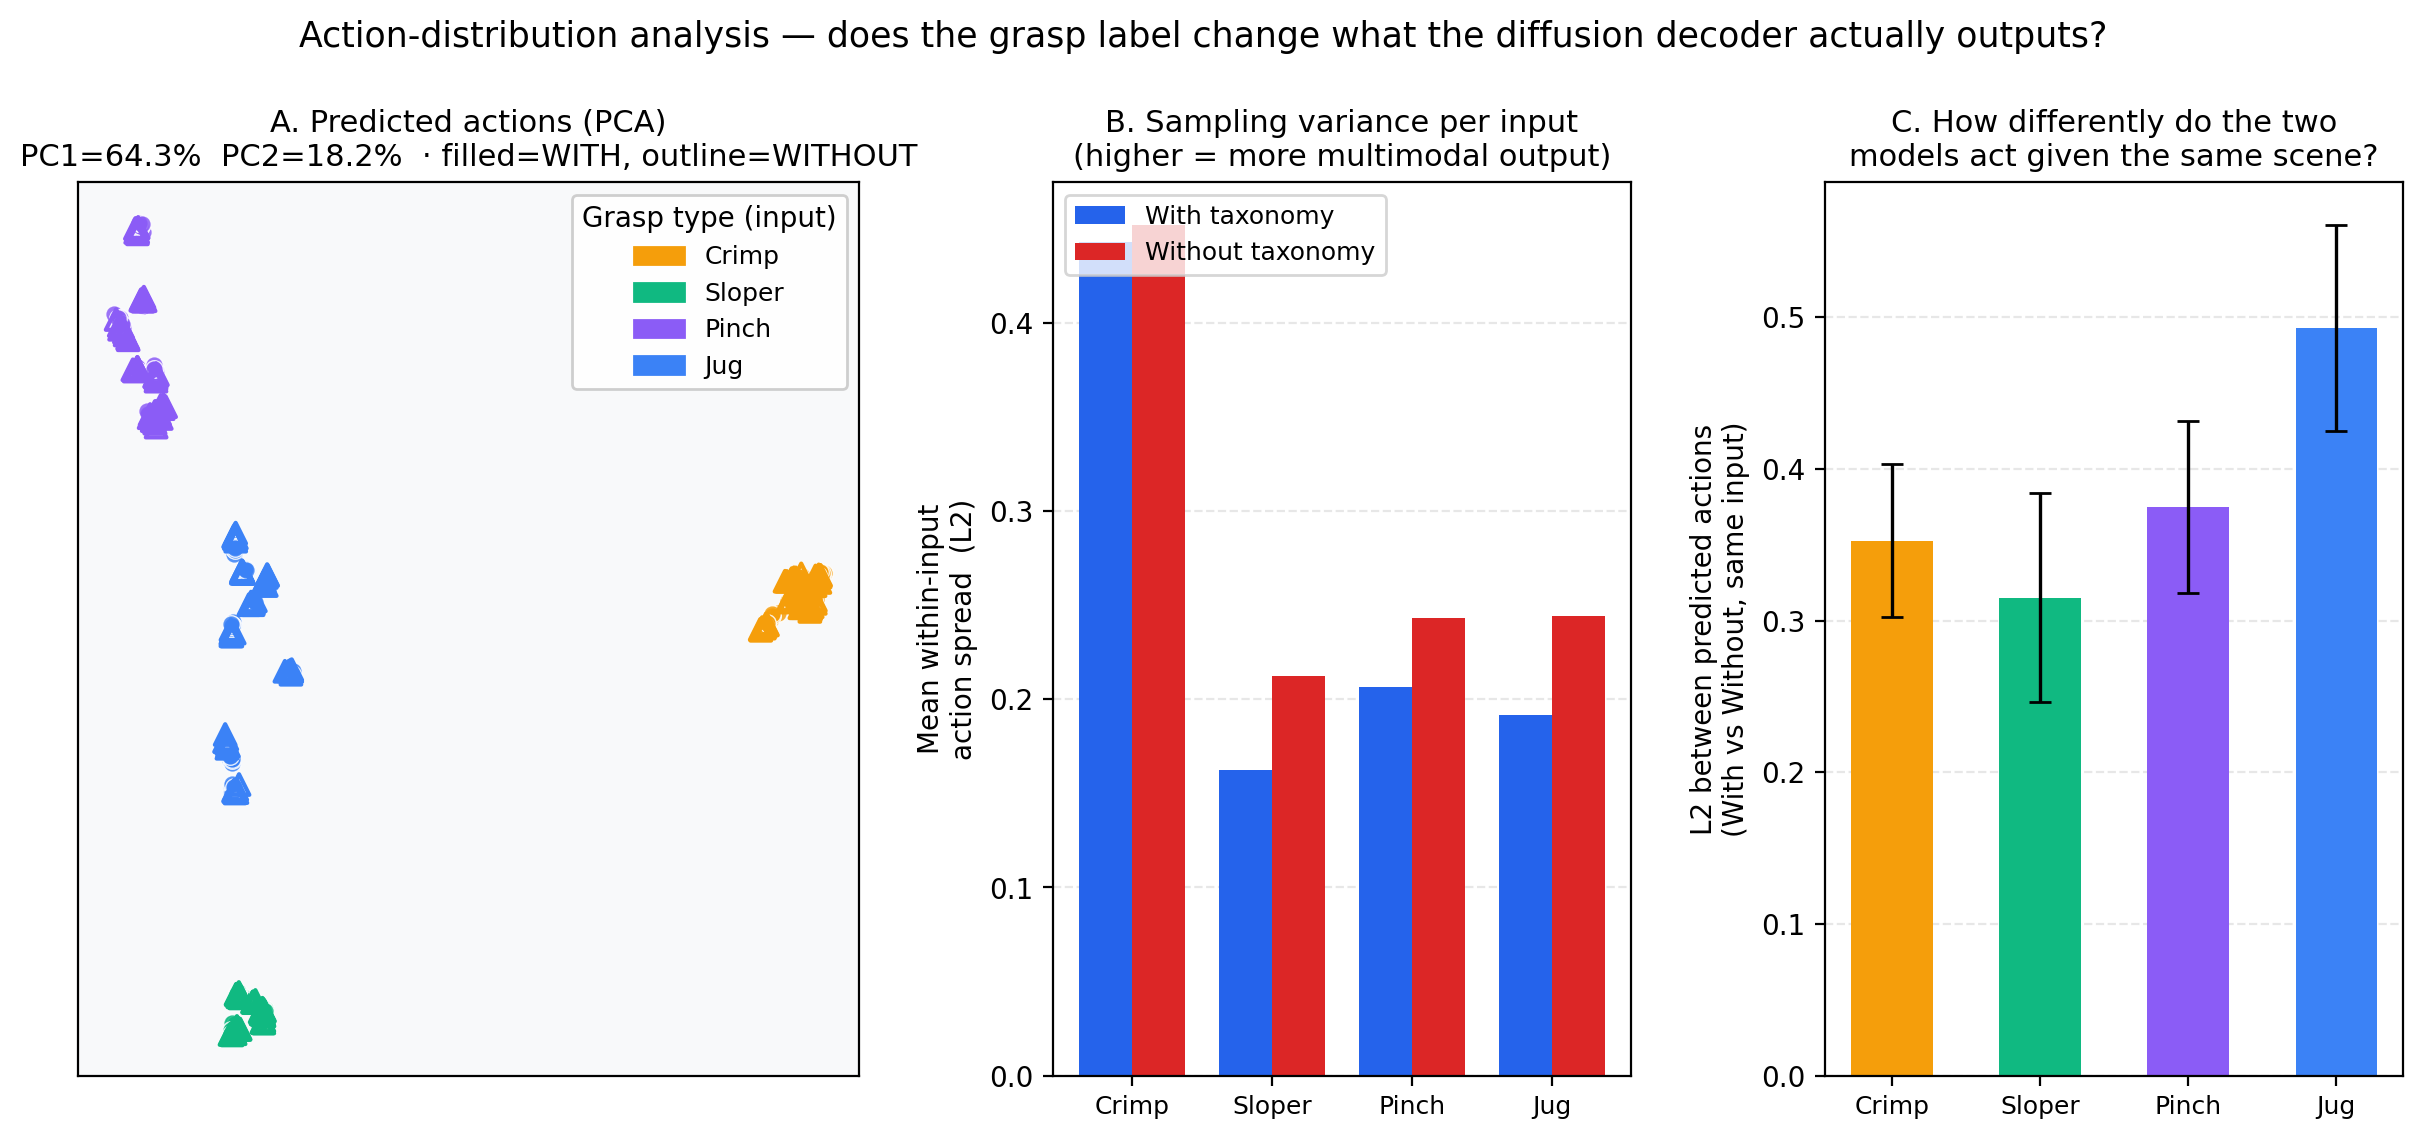
\includegraphics[width=\textwidth]{fig_action_distribution.png}
\caption{What the grasp label actually changes in the diffusion decoder
($K=8$ rollouts per input $\times$ 32 inputs per grasp type). (A) Predicted
actions in PCA: filled triangles (\emph{with} taxonomy) and outlined triangles
(\emph{without}) overlap closely per grasp type---both policies commit to the
same modal action. (B) Within-input sampling spread: the without-taxonomy
policy samples with 15--30\% higher action standard deviation on the
precision-critical types (crimp, sloper, pinch); jug is statistically
indistinguishable. (C) Mean L2 distance between the two models' predicted
actions on matched inputs is largest on jug---the only type where the two
policies actually disagree, not coincidentally the only type with mm-scale
contact slack.}
\label{fig:mech_var}
\end{figure}

\paragraph{Latent-space separation.}
We compute silhouette score and stratified 5-fold kNN accuracy on the fused encoder
output for the without-taxonomy policy using held-out inputs spanning all four grasp
types. Despite receiving no conditioning signal, the encoder reaches kNN accuracy
99\% and silhouette 0.32, indicating that grasp-type structure is already present in
the representation (Fig.~\ref{fig:mech_latent}C). The point-cloud branch alone does
not separate the types (Fig.~\ref{fig:mech_latent}A, silhouette $-0.03$); the
structure comes from the proprioception channel.

\paragraph{Mean action commitment.}
We compute the between-type spread of mean predicted final-step hand poses across all
four grasp types. The without-taxonomy policy produces means that differ across
types at 90\% of the demonstrator's between-type spread (0.316\,rad vs.\ 0.352\,rad
for demonstrators; the with-taxonomy policy produces 0.314\,rad). The unconditioned
policy does not collapse to a single behaviour mode.

\paragraph{Within-input sampling variance.}
The difference lies in the spread of individual rollouts around each conditional
mean. On precision-critical grasp types (crimp, sloper, pinch; sub-millimetre
contact tolerances), the without-taxonomy policy samples with 15--30\% higher
within-input standard deviation than the with-taxonomy policy. On the jug, whose
deep incut pocket gives millimetre-scale contact slack, the two policies are
statistically indistinguishable in within-input variance
(Fig.~\ref{fig:mech_var}B).

\paragraph{Interpretation: taxonomy as a precision regularizer.}
Together, these results rule out the mode-selector account: the unconditional
representation already commits to the correct mode, so the label cannot be routing
to it. The role left for the label is to tighten the diffusion decoder's sampling
distribution around that mode, reducing per-rollout variance. The closest analogues
are classifier-free guidance in image diffusion \citep{ho2022cfg}, which sharpens
per-pixel predictions without changing the modal image, and low-temperature sampling
in language models. The label is a precision knob, not a switch.

The account predicts a specific ordering across grasp types: conditioning should
help most where contact geometry is unforgiving (thin crimps, narrow pinches,
high-friction slopers) and least where it provides slack (jug). The hardware
evaluation in \S\ref{sec:robot_eval} reports this ordering.

\subsection{Hardware Evaluation}
\label{sec:robot_eval}
We ran 80 paired trials = 160 rollouts (4 paired trials per orientation $\times$ 5
orientations $\times$ 4 hold types) in a single $\sim$7-hour session with a single
operator. No trial pegged the ratchet at $n = 11$, so the dataset is free of
right-censoring. Statistical tests are Wilcoxon signed-rank (two-sided) per grasp
type with $n=20$ pairs each; effect sizes are Cohen's $d$ on paired differences.

\begin{figure}[t]
\centering
\includegraphics[width=0.95\textwidth]{fig_ratchet_1_boxplots.png}
\caption{Per-trial slip force on the spring testbed, with vs.\ without taxonomy
conditioning, by grasp type (20 paired trials per type, 80 total). Boxes are
IQR, white lines are medians. All four comparisons clear $p < 0.05$ (Wilcoxon
signed-rank); the effect-size ordering matches the contact-tolerance prediction
from \S\ref{sec:mechanistic}: pinch $d=1.82 >$ sloper $d=1.08 \approx$ crimp
$d=1.05 \gg$ jug $d=0.55$. The without-taxonomy sloper boxplot is degenerate
(all 20 trials at preload force $\approx 5.2$\,N)---a complete-failure mode the
conditioning rescues.}
\label{fig:boxplots}
\end{figure}

\paragraph{H1: median slip force.}
Taxonomy conditioning improves grip strength on every grasp type tested
(Table~\ref{tab:paired_eval}). Overall median slip force rises from 7.9\,N to
13.1\,N, a $+5.2$\,N (66\%) improvement (Wilcoxon $p < 0.001$,
Cohen's $d = 0.95$; Fig.~\ref{fig:boxplots}).

\begin{table}[h]
\centering
\caption{Paired evaluation on the spring testbed: 20 paired trials per grasp type,
Wilcoxon signed-rank, two-sided. Cohen's $d$ computed on paired differences;
pinch and crimp share the same $\Delta$ median but pinch's larger $d$ reflects
a tighter distribution of paired differences (20 of 20 conditioned wins, all positive).
*** $p<0.001$, ** $p<0.01$, * $p<0.05$.}
\label{tab:paired_eval}
\begin{tabular}{lccccc}
\toprule
Grasp type & WITH median & WITHOUT median & $\Delta$ median & Wilcoxon $p$ & Cohen's $d$ \\
\midrule
Crimp  & 15.7\,N & 9.2\,N  & $+6.5$\,N & 0.0007 & 1.05 *** \\
Jug    & 15.7\,N & 14.4\,N & $+1.3$\,N & 0.0278 & 0.55 *   \\
Sloper & 7.9\,N  & 5.2\,N  & $+2.6$\,N & 0.0012 & 1.08 **  \\
Pinch  & 15.7\,N & 9.2\,N  & $+6.5$\,N & $<$0.001 & 1.82 *** \\
\midrule
\textbf{Overall} & \textbf{13.1\,N} & \textbf{7.9\,N} & \textbf{$+5.2$\,N} & \textbf{$<$0.001} & \textbf{0.95 ***} \\
\bottomrule
\end{tabular}
\end{table}

\paragraph{H2: ordering across grasp types.}
The effect-size ordering matches the precision-regularizer prediction from
\S\ref{sec:mechanistic}. Pinch, the narrowest hold, shows the largest effect
($d = 1.82$), with the conditioned model winning all 20 pairs. Sloper ($d = 1.08$)
and crimp ($d = 1.05$) follow, both high-precision contact geometries. The jug,
whose deep incut pocket accommodates sub-centimetre positioning error, gives the
smallest effect ($d = 0.55$). Aggregating across types, the conditioned model wins
61 of 80 pairs, ties 14, and loses 5.

\paragraph{Failure-mode rescue.}
Bucketing each rollout into complete failure ($\le 5.3$\,N, preload only), weak grip
($5.3$--$13.5$\,N), moderate grip ($13.5$--$23.0$\,N), or strong grip ($> 23.0$\,N)
exposes where the conditioning gain lives. The bin boundaries correspond to
0, 1--3, 4--7, and $\ge 8$ ratchet teeth, respectively. Complete failures fall from 44\% of
trials without conditioning to 10\% with it (a $4.4\times$ reduction), and strong
grips rise from 1\% to 9\%. Most of the improvement comes from converting failed
trials into measurable grips, with smaller gains in the upper tail
(Fig.~\ref{fig:failure}). Taxonomy conditioning does not merely sharpen
successful grips; it rescues failures.

\begin{figure}[t]
\centering
\includegraphics[width=0.92\textwidth]{fig_obs_1_failure_modes.png}
\caption{Failure-mode breakdown per grasp type (W = with taxonomy, W/o =
without). Bars stack 20 trials per cell into four force regimes. The most
striking column is sloper W/o, where all 20 trials collapse to complete
failure---conditioning converts 13 of these into weak grips (7 remain at
preload). Pinch and jug show no complete failures with conditioning. Crimp under conditioning shows 6/20 strong grips
versus 1/20 without. Across all four grasp types, conditioning reduces
complete failures from 44\% $\to$ 10\% and raises strong grips from 1\% $\to$ 9\%.}
\label{fig:failure}
\end{figure}

\paragraph{Orientation profile.}
Per-orientation breakdown shows the expected geometric pattern: performance peaks
near $0^\circ$ (pull-aligned) and degrades as the hold rotates toward $\pm 45^\circ$,
where the moment arm between contact and pull axis maximises mechanical disadvantage
against the grip. Crimp shows the largest orientation sensitivity (18\,N spread
between hardest and easiest orientation), consistent with the thin lateral profile of
the crimp edge providing little angular tolerance; pinch and jug exhibit a more
uniform response with the aligned ($0^\circ$) case strongest
(Fig.~\ref{fig:orientation}).

\begin{figure}[t]
\centering
\includegraphics[width=\textwidth]{fig_ratchet_8_orientation_heatmap.png}
\caption{Mean slip force (N) per grasp type $\times$ hold orientation, each
cell averaged over 4 paired trials. Darker = stronger grip. The with-taxonomy
heatmap (blue) is strictly stronger than without-taxonomy (red) in every cell.
Crimp shows the largest orientation sensitivity: $27$\,N at $-22.5^\circ$
versus $8$\,N at $+45^\circ$. The sloper row of the without-taxonomy heatmap
is flat at 5\,N---uniform complete failure across all orientations.}
\label{fig:orientation}
\end{figure}

\paragraph{Methodological controls.}
Strict global order alternation made each model run first in exactly 40 of 80 pairs.
A Mann--Whitney $U$ test between when-first and when-second rollouts found no
detectable order bias for either model (with $p = 0.771$, without $p = 0.690$),
confirming the alternation protocol absorbed any session-level drift. A fresh fused
point cloud was captured before every single rollout (not shared within a pair);
the median between-trial PC centroid drift was sub-millimetre, well below the
post-hoc 15\,mm drift filter threshold, and no pairs were dropped.

% -----------------------------------------------------------------------
\section{Discussion}
\label{sec:discussion}
% -----------------------------------------------------------------------

\paragraph{Taxonomy conditioning as a precision regularizer.}
The mechanistic findings in \S\ref{sec:mechanistic} shift the standard reading of why
taxonomy conditioning helps. Prior work on conditional generative models often treats
the conditioning signal as a mode selector. For a dexterous diffusion policy trained
on a mixed-grasp dataset, the mode is already selected by the unconditional
representation; the label's contribution is a reduction in sampling variance. The
geometric prediction follows directly: the variance-reduction effect should help
where contact tolerances are tight (thin crimps, narrow pinches, high-friction
slopers) and be irrelevant where the geometry supplies slack (deep jug pockets). The
Cohen's $d$ values recovered in \S\ref{sec:robot_eval} (pinch 1.82, sloper 1.08,
crimp 1.05, jug 0.55) reproduce this ordering without per-type tuning.

Classifier-free guidance \citep{ho2022cfg} offers the closest analogue. CFG in image
diffusion does not change the modal image; it sharpens detail and reduces variance
around the mode. The taxonomy label here plays the same role for the joint-space
action distribution.

\paragraph{Failure-mode rescue as the dominant mechanism.}
The gain from conditioning is concentrated in the lower tail of the slip-force
distribution. The unconditioned policy degenerates to no-contact behaviour
(complete failure, force at preload only) on 44\% of trials; the conditioned policy
shows this mode on 10\%. The precision-regularizer view supplies a simple
explanation: when sampling variance exceeds the geometric contact tolerance, each
draw is rolled against the failure region, and shrinking the variance shrinks the
failure-set probability mass. Improvements elsewhere in the distribution are
secondary to this lower-tail rescue.

\paragraph{Benchmark design.}
The spring displacement testbed provides experimental control unavailable in standard
pick-and-place lift tests: the pull direction and magnitude are fixed by hardware,
and the ratchet gives a continuous reading rather than a threshold-dependent binary.
Testing at five hold orientations isolates the effect of grip approach angle from
grasp quality, enabling profile plots across angles rather than a single aggregate
success rate.

\subsection{Limitations}
\label{sec:limitations}

\paragraph{Single demonstrator, single hold per type.}
All 200 training episodes come from one operator and one teleop session, and
each grasp category is represented by exactly one physical hold. The per-type
effect sizes reported here therefore conflate ``the precision regularizer effect
on that grasp type'' with ``the precision regularizer effect on this hold.''
A held-out crimp variant (\textit{test\_edge}) is collected but not evaluated
in this paper.

\paragraph{Single platform.}
Franka + LEAP only. The qualitative claim---the label tightens an
already-committed mode rather than selecting one---should be architecture-general
for diffusion policies on mixed-grasp datasets, but the specific Cohen's $d$
values are platform-specific until shown otherwise.

\paragraph{Single-axis proxy.}
The spring testbed measures grip force against displacement on one fixed axis.
This captures the dominant load direction of dynamic crux moves but not
multi-directional or sustained loads. The ratchet truncates above
$\sim 33.9$\,N; no trial in this session reached the ceiling, so the present
analysis is censoring-free.

\paragraph{Single seed.}
Training did not pin a global random seed. The qualitative findings are robust
given the Cohen's $d$ range (0.55--1.82), but seed-averaged numbers belong in a
final revision. The planned wrong-label ablation---feeding the conditioned
policy a deliberately mismatched label to test causality---is not yet run.

\paragraph{Single-session evaluation.}
80 paired trials in one $\sim$7-hour session, one rater. Strict global
alternation absorbed session-level drift inside the comparison
(\S\ref{sec:robot_eval}); inter-session variance is uncharacterised.

\paragraph{Orientation not in the observation.}
Hold orientation is logged per pair but not stored in the training zarr; the
policy infers it from the point cloud. Whether explicit orientation conditioning
would shrink the 18\,N crimp range across orientations is open, but orientation
is not realistically available at deployment without auxiliary perception.

\paragraph{Absolute grip quality.}
Median slip force with conditioning is 13.1\,N---moderate, not strong. The gain
is overwhelmingly a failure-mode rescue (complete-failure rate 44\% $\to$ 10\%)
rather than a strong-grip producer; the strong-grip rate of 9\% leaves obvious
headroom for per-grasp specialisation, data scaling, or contact-aware auxiliary
losses.

% -----------------------------------------------------------------------
\section{Conclusion}
% -----------------------------------------------------------------------
We presented CRAG, a grasp-taxonomy-aware 3D diffusion policy for dexterous
climbing hold manipulation, together with a climbing-hold benchmark on a
spring-constrained displacement testbed instrumented with a linear ratchet that
yields a continuous slip-force readout. The central finding is mechanistic:
taxonomy conditioning in a dexterous diffusion policy functions as a
\textbf{precision regularizer}. The unconditioned policy already separates grasp
types in representation (kNN 99\%, silhouette 0.32) and commits to type-distinct
mean actions at 90\% of demonstrator spread; the taxonomy label contributes a
15--30\% reduction in within-input sampling variance on precision-critical grasp
types.

Hardware evaluation on 80 paired trials supports this account. Median slip force
rises by 5.2\,N with conditioning (Wilcoxon $p < 0.001$, Cohen's $d = 0.95$), and
effect sizes are ordered by contact-tolerance tightness (pinch 1.82, sloper 1.08,
crimp 1.05, jug 0.55). The largest single effect is on the lower tail: the
complete-failure rate falls from 44\% of trials to 10\%. Strict global
order alternation with per-trial point-cloud capture rules out order bias and
hold drift as alternative explanations.

\paragraph{Reproducibility.}
Everything needed to redo both training and the paired evaluation is released.
The two checkpoints (with and without taxonomy) are a matched ablation pair:
34{,}621{,}365 and 34{,}584{,}117 parameters, identical except for the
grasp-type encoder branch (\S\ref{sec:arch}). All figures in this paper
regenerate from the released evaluation JSON via the included analysis scripts.
Training did not pin a global random seed, so bitwise reproducibility from the
code alone is not achievable in the current run---the published checkpoints
are the canonical artifacts. The spring testbed is custom; CAD, 3D-print files,
and a parts list with commercial-equivalent spring specifications will be
released on acceptance.
\begin{itemize}[leftmargin=*,topsep=2pt,itemsep=1pt]
  \item Code: \url{https://github.com/<anonymized for review>}
  \item Training data: \texttt{<anonymized>/climbing-holds-pointcloud} (rig version, 200 episodes, 27{,}821 timesteps)
  \item Checkpoints: \texttt{<anonymized>/climbing-holds-rig-\{with,no\}-taxonomy}
  \item Evaluation session: \texttt{paired\_session\_20260515\_074256.json}
  \item Analysis scripts: \texttt{eval\_results/\{generate\_ratchet\_figures,generate\_training\_curves,display\_results,analyze\_observations\}.py}
\end{itemize}

% Flush all main-text floats here so none drift past the conclusion.
\FloatBarrier

\appendix
% -----------------------------------------------------------------------
\section{Supplementary Figures}
% -----------------------------------------------------------------------

\begin{figure}[h]
\centering
\includegraphics[width=\textwidth]{fig_latent_4panel.png}
\caption{Learned representations across four embedding levels (t-SNE of training
episodes, coloured by grasp type), referenced in \S\ref{sec:mechanistic}.
(A) The raw PointNet geometry embedding is not separable (silhouette $-0.03$,
5-NN $39\%$): the four hold geometries are not natively distinguishable from
cropped point clouds alone. (B,C) Both the \emph{with}-taxonomy and
\emph{without}-taxonomy fused encoder outputs (PC $+$ state, with or without
the grasp label) recover near-identical separation (silhouette $0.33$ vs.\
$0.32$, 5-NN $99.5\%$ vs.\ $99\%$). The label is not what creates the
grouping---proprioception is. (D) Joint trajectories show the same clusters in
the action space.}
\label{fig:mech_latent}
\end{figure}

\bibliographystyle{plainnat}
\bibliography{references}

\end{document}
